\newpage
\section{センサーボードを使ってみよう}
センサーボードとは、ラズベリーパイの上部に\ruby{接続}{せつ|ぞく}することでラズベリーパイで出来ることを\ruby{拡張}{かく|ちょう}するための\ruby{基板}{き|ばん}です。子ども IT \ruby{未来塾}{み|らい|じゅく}では Indoor Corgi Elec. という会社が\ruby{販売}{はん|ばい}している RPZ-IR-Sensor を使います。下記 URL から販売ページを見ることができます。これを使うことで、例えばスイッチを使ったり、温度や\ruby{湿度}{しつ|ど}を\ruby{計測}{けい|そく}したり、赤外線で動く家電を\ruby{操作}{そう|さ}したりすることができるようになります。\\
\url{https://www.indoorcorgielec.com/products/rpz-ir-sensor/}\\

% \begin{figure}[H]
%     \centering
%     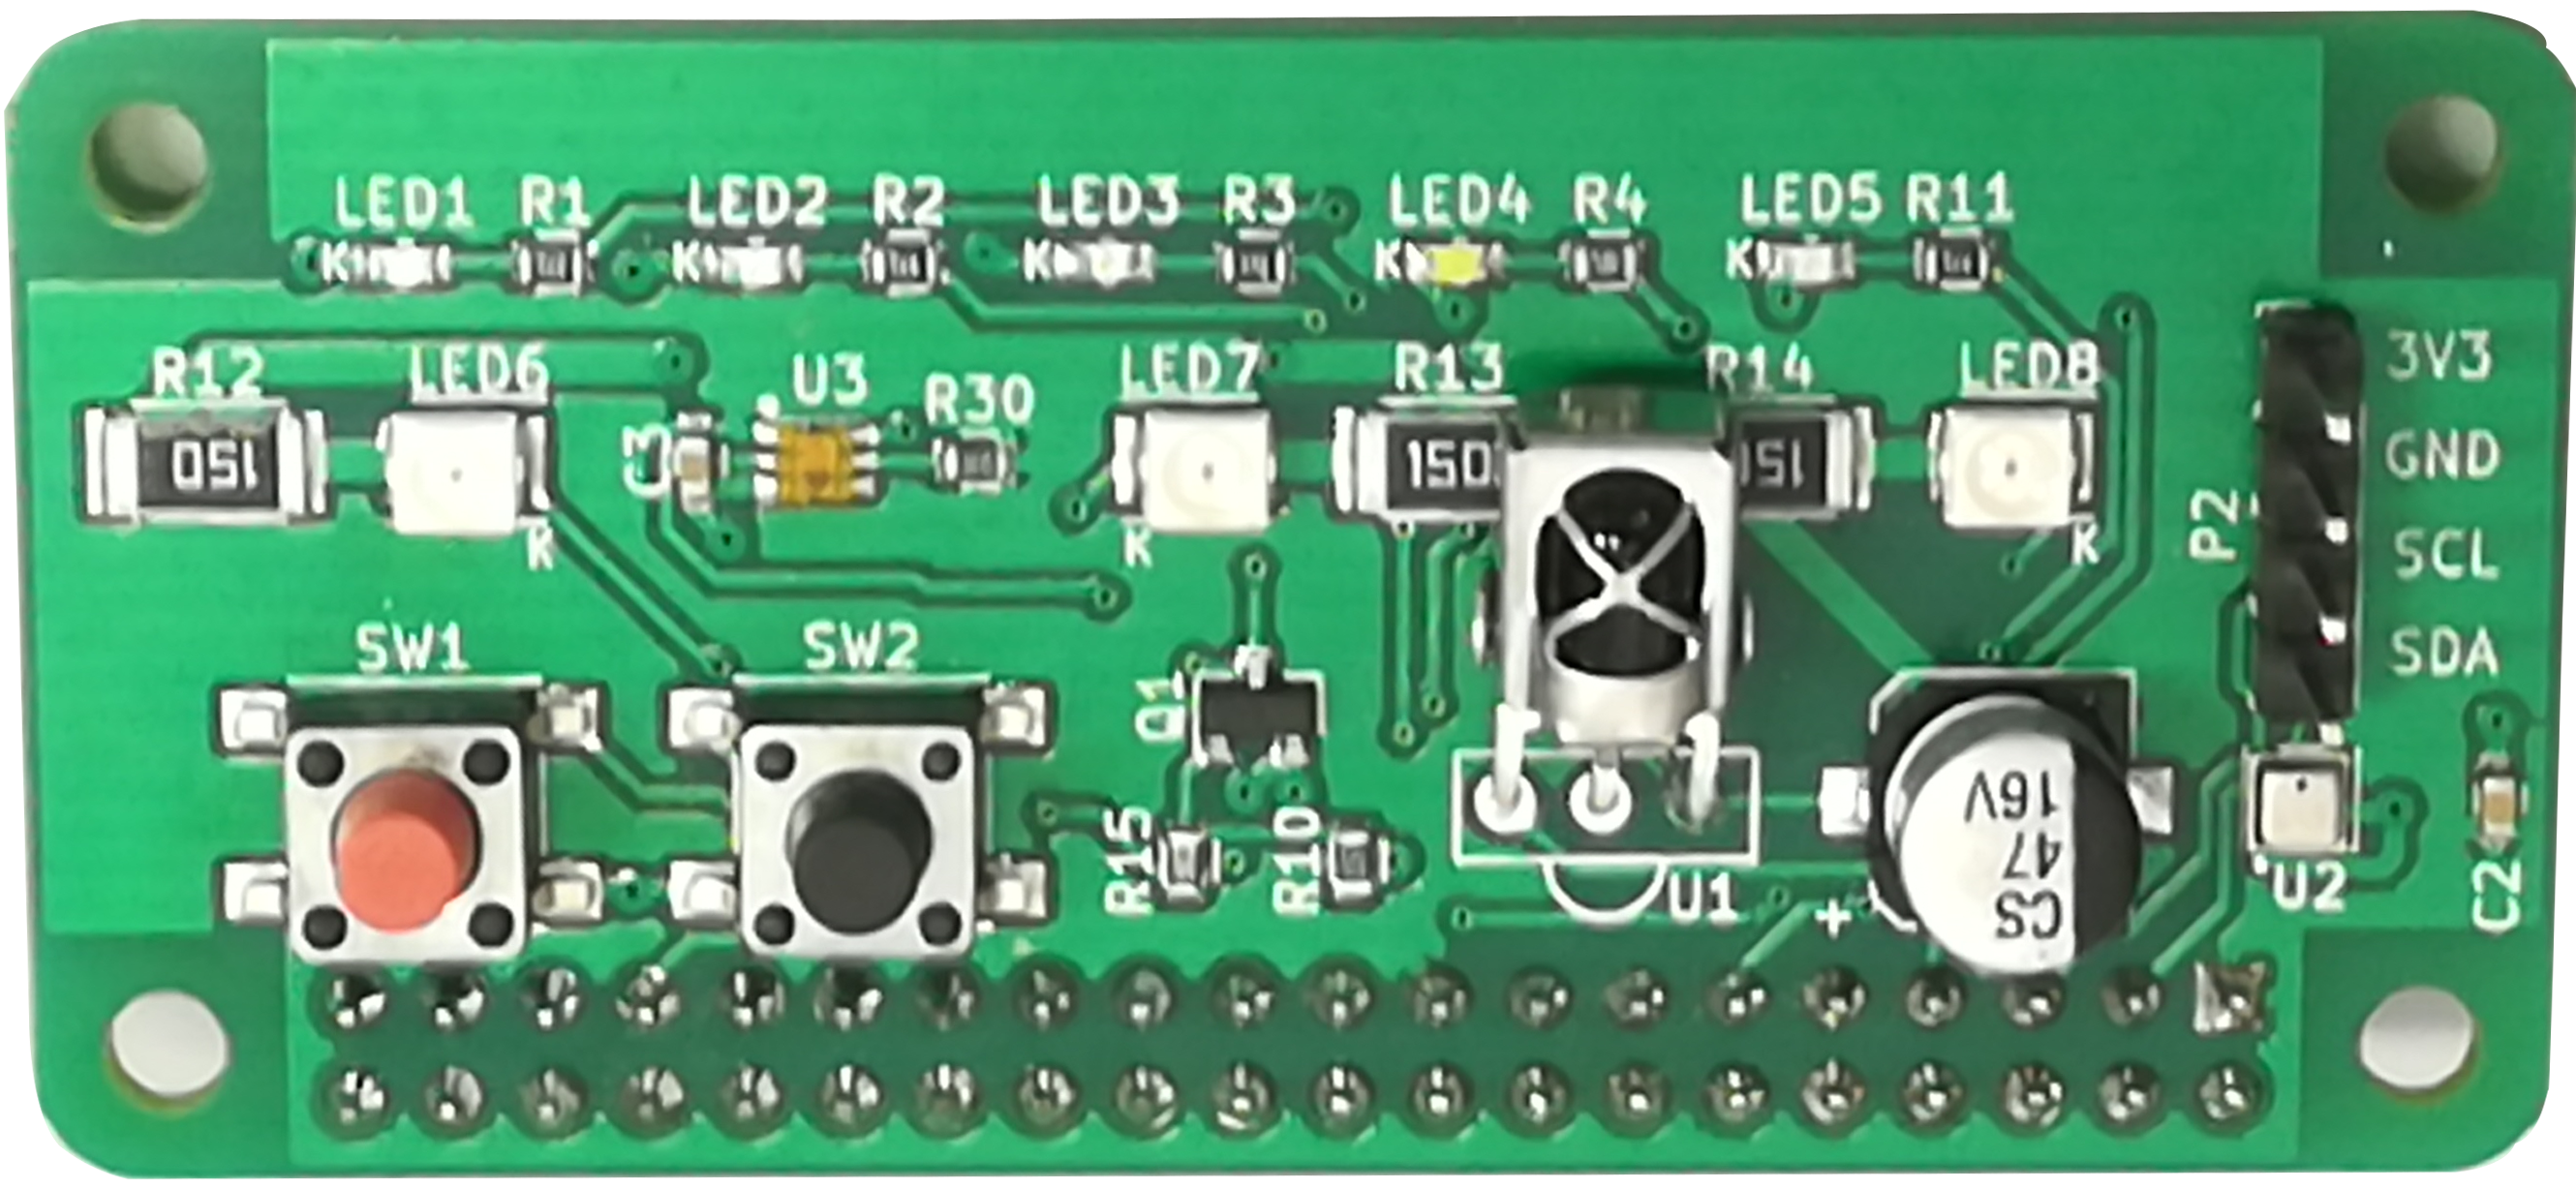
\includegraphics[width=0.6\linewidth]{images/chap03/text03-img030.png}
%     \caption{センサーボード}
% \end{figure}

温湿度\ruby{気圧}{き|あつ}センサーはセンサーボード上に取り付けられたセンサーと、外付けのセンサーの2種類があります。センサーボード上のセンサーがラズベリーパイの熱のせいで熱くなってしまうので、基本的には外付けのセンサーを使いましょう。

外付けセンサーを取り付けるときはピンに正しい向きがあるので、赤い線が3V3にささるように、下の写真のように取り付けてください。外付けセンサーとセンサーボードの金属部分同士が触れると、大きな電流が流れて危険な事故につながります。十分に気を付けましょう。

\begin{figure}[H]
    \centering
    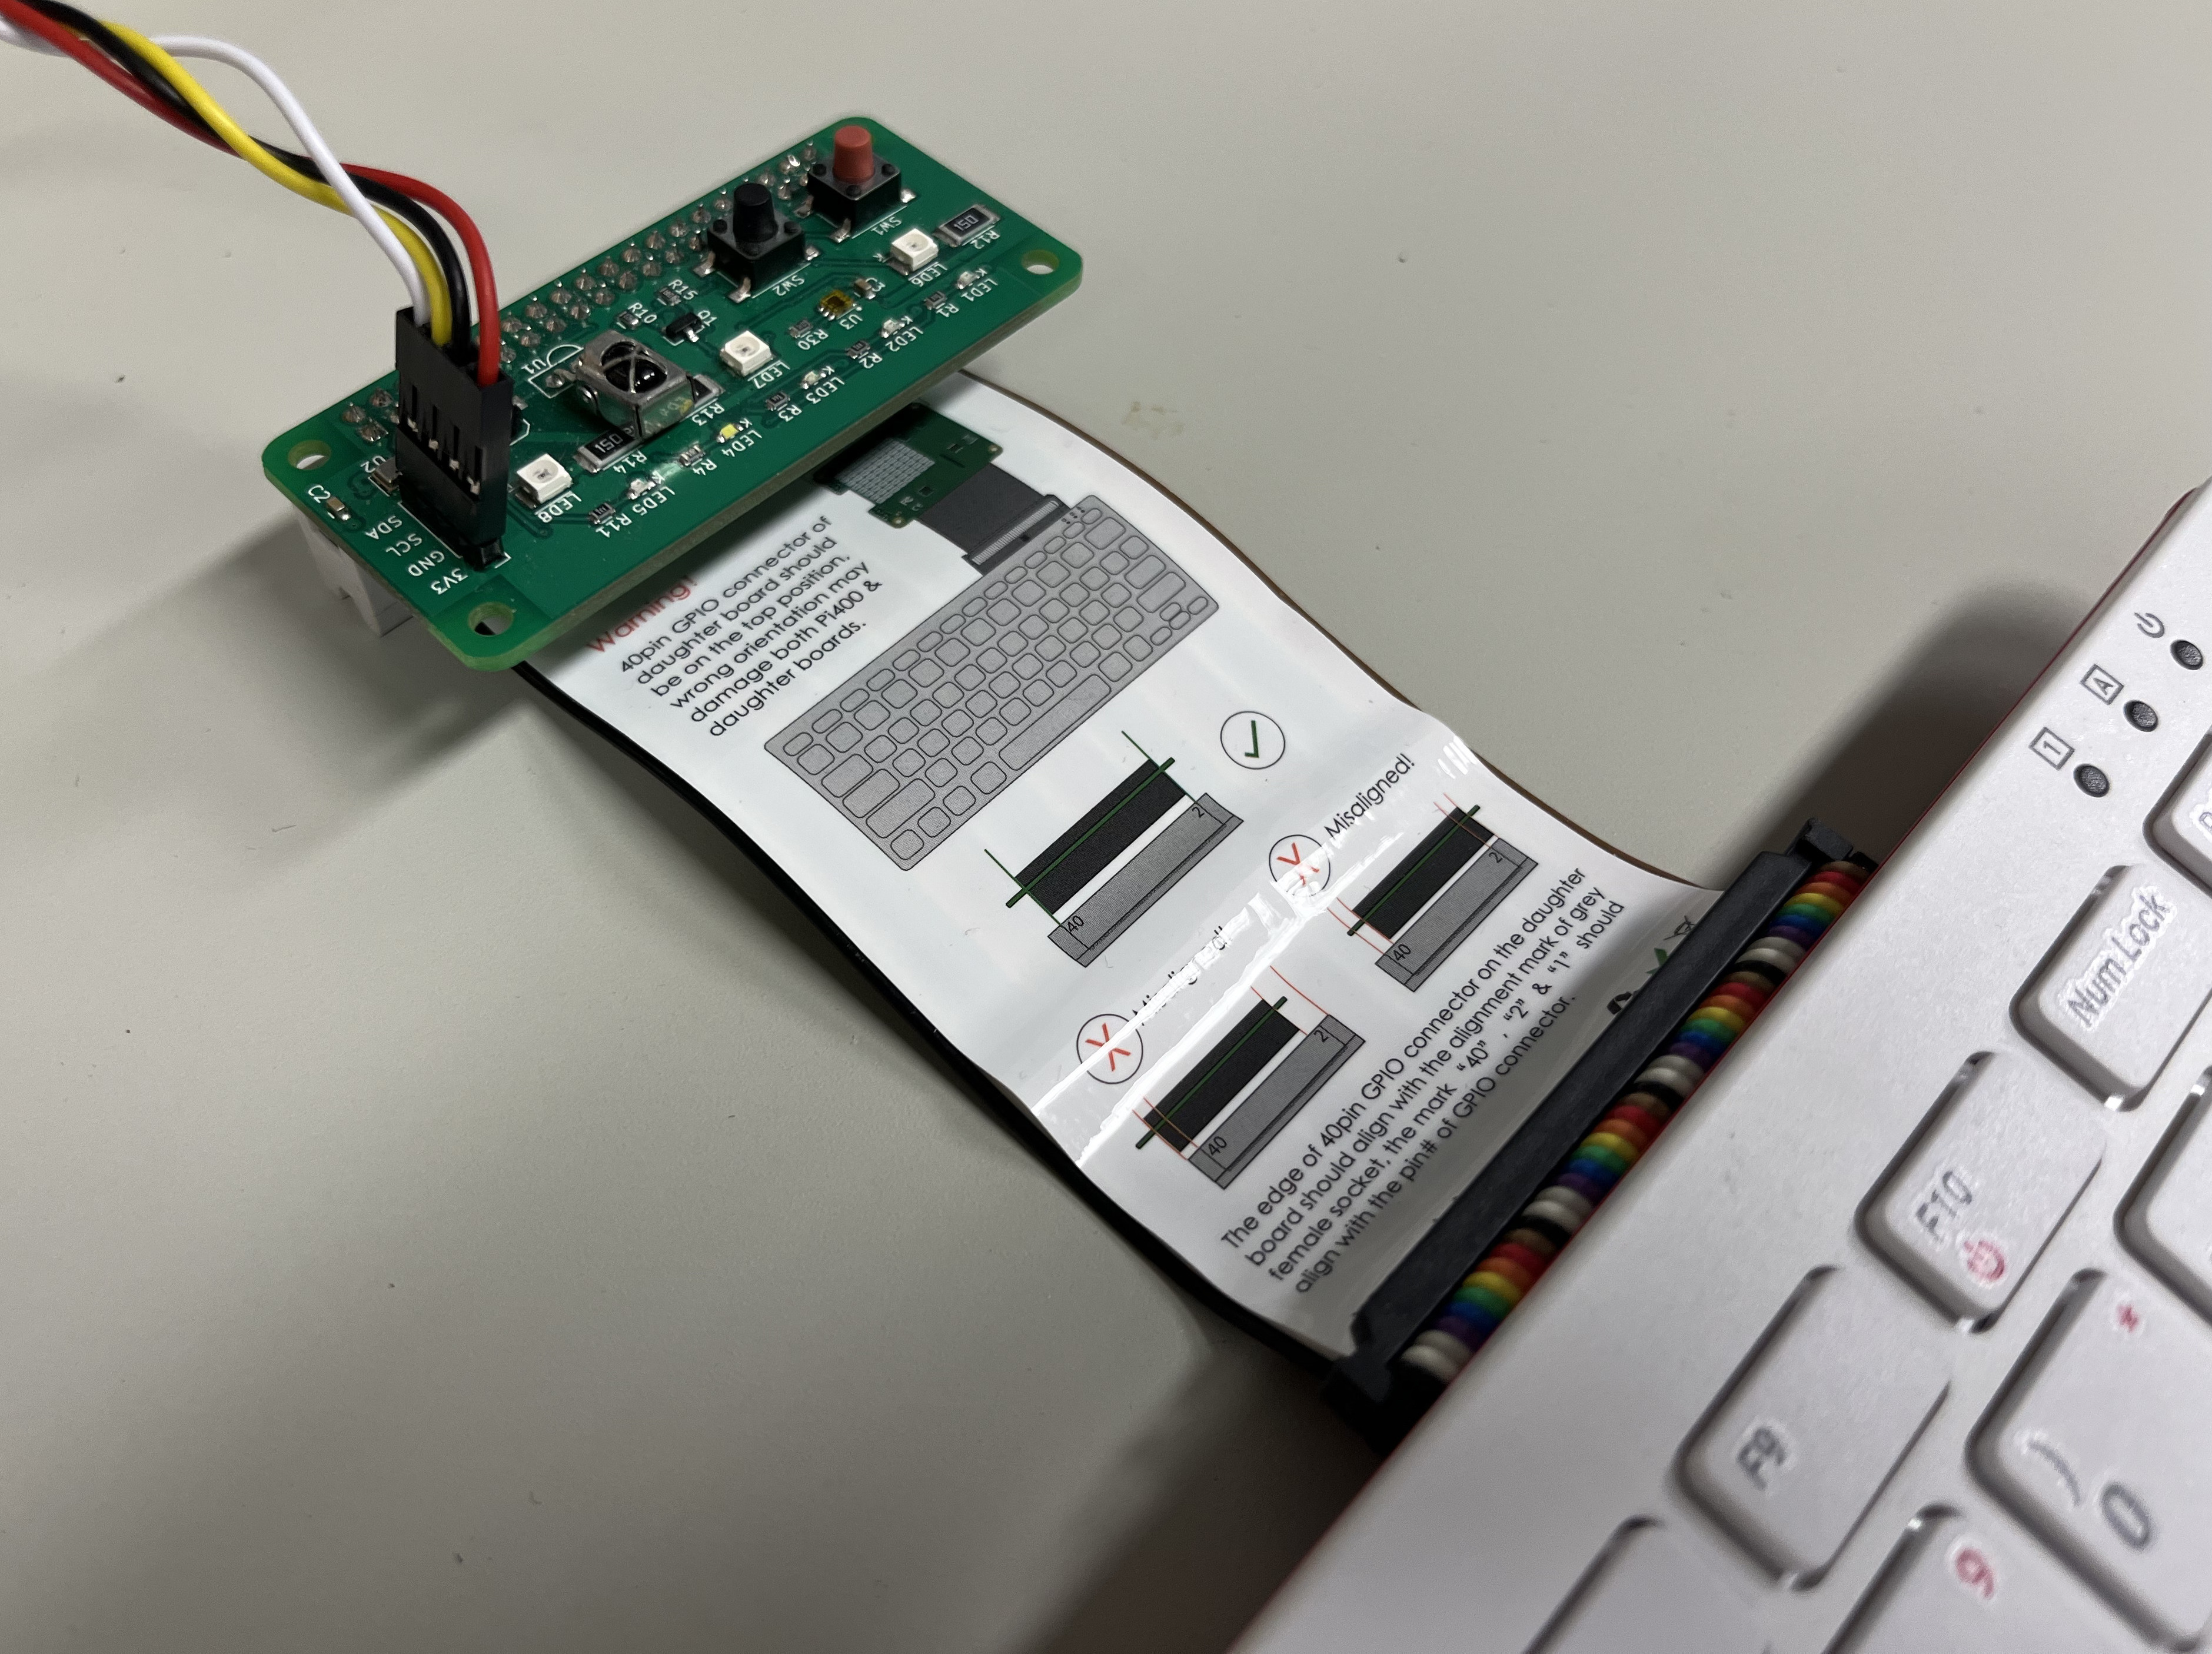
\includegraphics[width=0.6\linewidth]{images/chap03/how_to_install_bme280.jpg}
    \caption{外付けセンサーの取り付け方法}
\end{figure}

\section{センサーボードとGPIO}
センサーボードとラズベリーパイは図\ref{sensors}のように接続されています。たとえば LED1 を使いたいときは GPIO17 というピンを使います。

\begin{figure}[H]
    \centering
    \includesvg[width=\linewidth]{images/chap03/rpz-ir-sensor.svg}
    \caption{センサーボードとラズベリーパイのかんけい}
    \label{sensors}
\end{figure}



% 消去予定
% \section{LEDの点灯・消灯を\ruby{制御}{せい|ぎょ}してみよう}
% \subsection{LED を光らせよう}

% まずはセンサーボードにある LED を光らせてみましょう。HSP スクリプトエディタから LED を光らせるプログラム(led.hsp)を読み\ruby{込}{こ}んで実行してみましょう。led.hsp は、\textasciitilde /03のディレクトリにあります。\\

% \begin{lstlisting}[caption=\textasciitilde/03/led.hsp,label=led.hsp]
% #include "hsp3dish.as"		<#blue#;スクリプトの設定を読み込む#>
% #include "rpz-gpio.as"		<#blue#;スクリプトの設定を読み込む#>
% 	redraw 0		<#blue#;画面更新(仮想画面に描画)#>
% 	font "",30		<#blue#;文字のフォント、サイズを決める#>
% 	pos 20,20		<#blue#;文字の場所を決める#>
% 	mes "LED が光るよ"	<#blue#;文字を決める#>
% 	redraw 1		<#blue#;画面更新(実際の画面に描画)#>
% *led
% 	gpio 17, 1		<#blue#;GPIO17 を点灯させる#>
% 	wait 100		<#blue#;0.1 秒待つ#>
% 	goto *led		<#blue#;*led まで戻る#>
% 	gpio 17, 0		<#blue#;GPIO17を消灯させる#>
% \end{lstlisting}

% 下の写真のように LED が光りましたか?\\

% \begin{figure}[H]
%     \centering
%     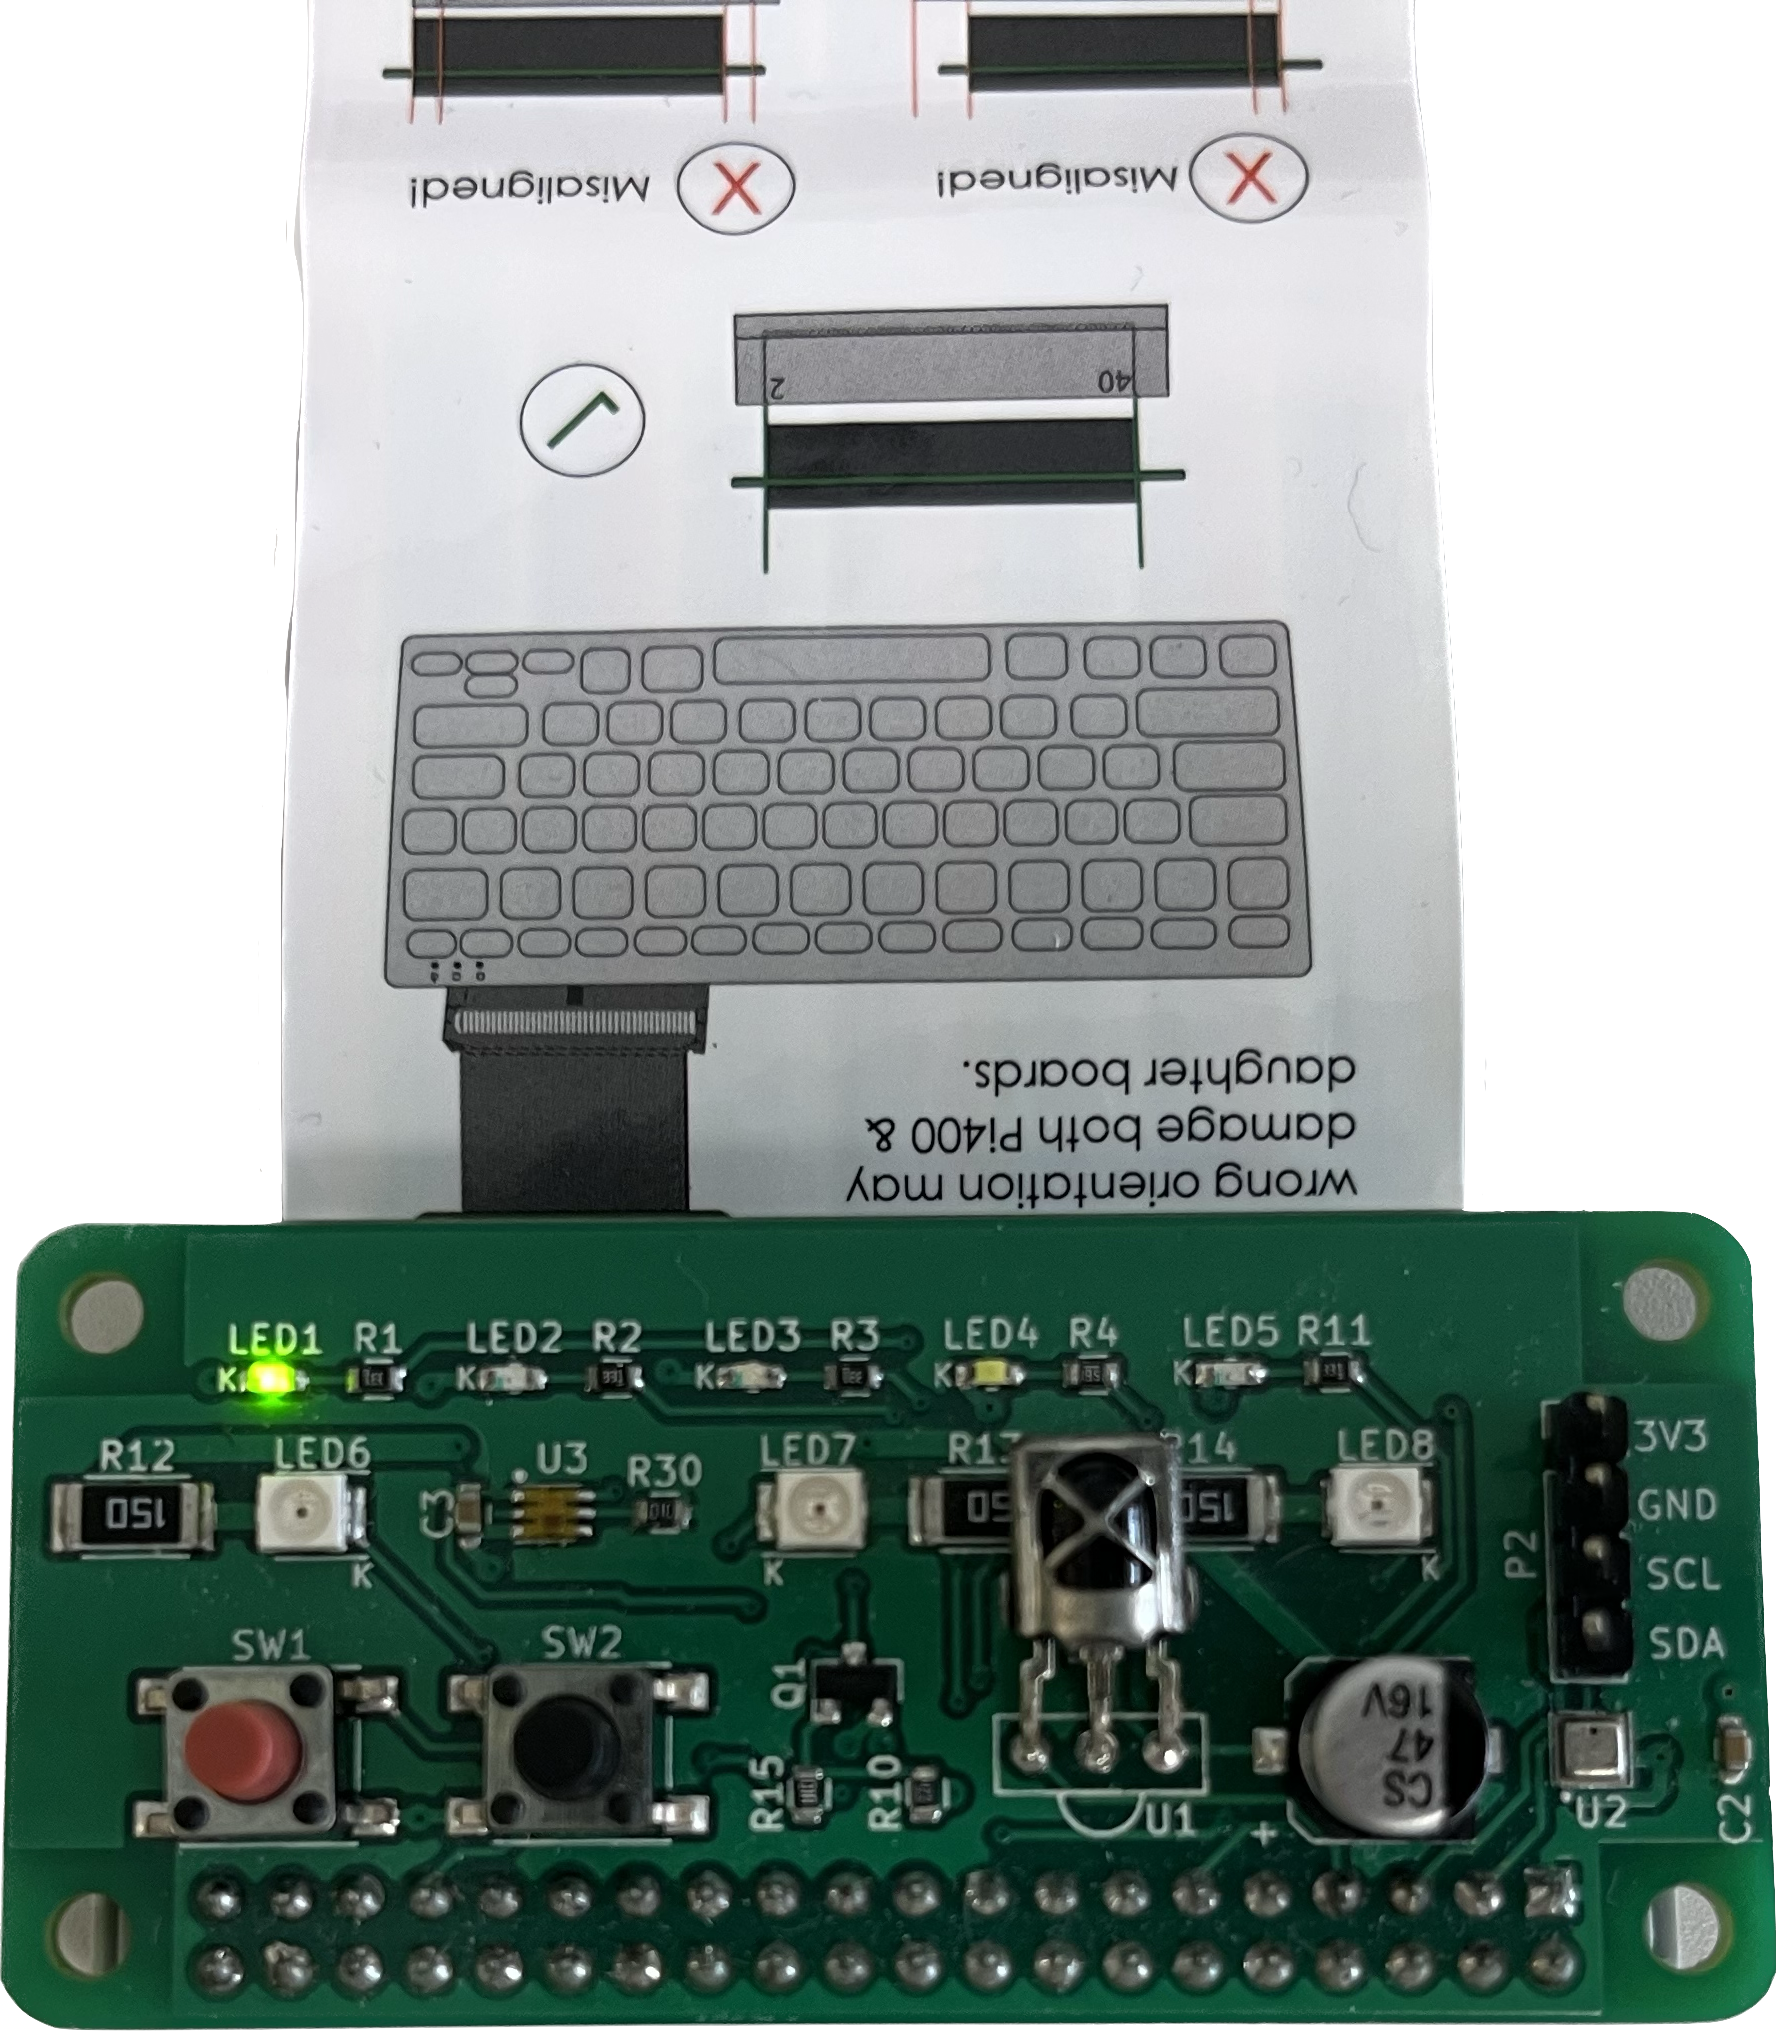
\includegraphics[width=0.5\linewidth]{images/chap03/led_emission_demo.png}
% \end{figure}

% それではプログラムを\ruby{解析}{かい|せき}してみましょう。\code{font} 命令や \code{pos} 命令、 \code{mes} 命令がありますね。これらがどんな命令だったかを前回の教科書を読んで\ruby{復習}{ふく|しゅう}しましょう。gpio 命令も前回勉強しました。17という数字は上の図\ref{sensors}の GPIO17 に\ruby{対応}{たい|おう}していて、1 という数字は ON をあらわすのでしたね。\\

% \begin{tcolorbox}[title=\useOmetoi]
% \begin{enumerate}
% \addquiz{緑色のLED を光らせる命令を書きましょう(ヒント: 教科書第 2 回 2.3.3 LED がてんめつするスクリプトを参考にしましょう)。}
% \addquiz{緑色のLED を消す命令を書きましょう(ヒント: 教科書第 2 回 2.3.3 LED がてんめつするスクリプトを参考にしましょう)。}
% \addex{ターミナルを使って led.hsp のコピーを、321.hsp という名前で作りましょう。}
% \addex{他の色の LED が光るように 321.hsp のプログラムを変えてみましょう。}
% \end{enumerate}
% \end{tcolorbox}

